\subsection{Spectral Scaling and the Projection Ontology}
  \label{subsec:spectral-scaling-projection-ontology}

  The preceding derivation of the mass ratio $m_p/m_e$ rests on a fundamental shift in the ontology of mass.
  Within the Cosmochrony framework, inertial mass is no longer treated as an
  intrinsic ``charge'', but as a spectral signature of projection visibility.

  \paragraph{Mass as Spectral Weight}
    The non-injective nature of the projection $\Pi$ (see Section~\ref{subsec:intrinsic-structural-indeterminacy})
    implies that any effective particle in $\chi_{\mathrm{eff}}$ corresponds to a large
    equivalence class of micro-configurations in the substrate $\chi$.
    The stability eigenvalues $\lambda_n$ of the operator $L_{\mathrm{sol}}$ can
    therefore be reinterpreted as a coarse-grained measure of this structural multiplicity, or \emph{fiber weight}.
    A configuration that requires a larger set of internal modes to remain stable
    and projectable manifests a higher resistance to global relaxation, and thus a higher inertial mass.

  \paragraph{Invariance of the Ratio}
    Since the ratio
    \begin{equation}
      \frac{m_p}{m_e} \;\approx\; \sqrt{\frac{\lambda_p}{\lambda_e}}
    \end{equation}
    is independent of the absolute action scale $\hbar_\chi$, it is identified as a
    structurally protected invariant of the projection process itself.
    This explains the observed universality of the proton-to-electron mass ratio
    across cosmological epochs, regardless of the global relaxation state of $\chi$.

  \paragraph{The Spectral Packing Fraction ($\alpha$)}
    The hierarchy between the composite sector (proton) and the elementary sector
    (electron) is encapsulated by the spectral packing fraction
    \begin{equation}
      \alpha \;\equiv\; \frac{\lambda_e}{\lambda_{\mathrm{bind}}}
      \;\approx\; 3 \times 10^{-7}.
    \end{equation}
    Rather than an empirical fit, $\alpha$ represents the ratio of spectral
    transmittance under $\Pi$.
    The proton is heavy because its non-trivial topology ($Q=3$) constrains the
    stability operator $L_{\mathrm{sol}}$ to exhibit a large internal spectral bandwidth.
    This topological constraint, often heuristically represented by a trefoil-knot
    configuration, leads to a strong spectral gap between the binding modes
    $\lambda_{\mathrm{bind}}$ and the fundamental electronic mode $\lambda_e$.

  \paragraph{Conclusion}
    While the precise numerical value $m_p/m_e \simeq 1836$ awaits a closed-form
    derivation from the spectral geometry of $L_{\mathrm{sol}}$ on topologically
    constrained manifolds, the Cosmochrony framework reformulates the mass-ratio
    problem in structural terms.
    The proton-to-electron mass ratio emerges as the macroscopic signature of a
    spectral gap dictated by the complexity of the substrate’s excitations under
    projection, as schematically illustrated in Fig.~\ref{fig:spectral-gap},
    rather than as an arbitrary fundamental constant.

    \begin{figure}[htbp]
      \centering
      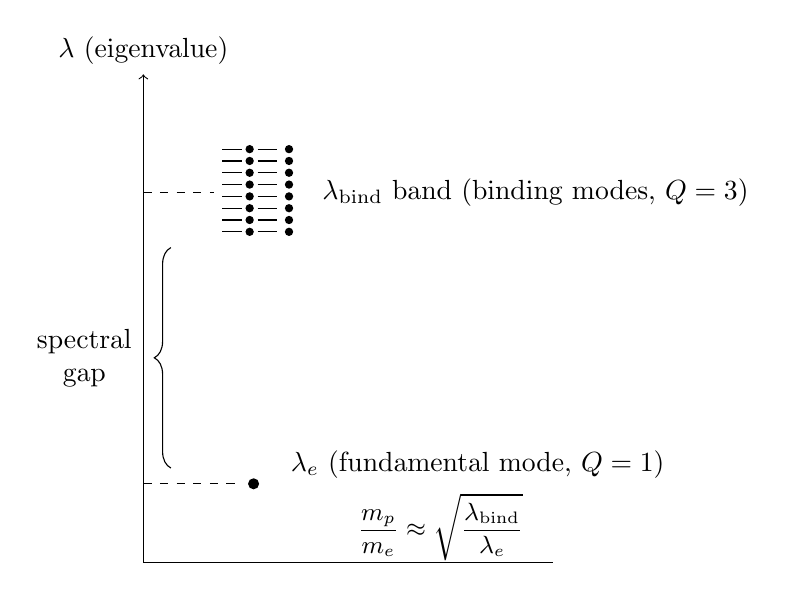
\begin{tikzpicture}[x=1cm,y=1cm]
      % Axis
      \draw[->] (0,0) -- (0,6.2) node[above] {$\lambda$ (eigenvalue)};
      \draw (0,0) -- (5.2,0);

      % Electron fundamental mode lambda_e
      \fill (1.4,1.0) circle (2pt);
      \node[anchor=west] at (1.75,1.25) {$\lambda_e$ (fundamental mode, $Q=1$)};

      % Binding band near lambda_bind
      \foreach \y in {4.2,4.35,4.5,4.65,4.8,4.95,5.1,5.25} {
        \draw (1.0,\y) -- (1.25,\y);
        \fill (1.35,\y) circle (1.5pt);
        \draw (1.45,\y) -- (1.70,\y);
        \fill (1.85,\y) circle (1.5pt);
      }
      \node[anchor=west] at (2.15,4.7) {$\lambda_{\mathrm{bind}}$ band (binding modes, $Q=3$)};

      % Indicate the gap with a brace
      \draw[decorate,decoration={brace,amplitude=6pt}]
      (0.35,1.2) -- (0.35,4.0)
      node[midway,xshift=-1.1cm,align=center] {spectral\\gap};

      % Optional dashed guide lines
      \draw[dashed] (0,1.0) -- (1.2,1.0);
      \draw[dashed] (0,4.7) -- (0.9,4.7);

      % Formula moved to the bottom-right (no overlap)
      \node[anchor=west,align=left] at (2.6,0.45)
        {\small $\displaystyle \frac{m_p}{m_e}\approx \sqrt{\frac{\lambda_{\mathrm{bind}}}{\lambda_e}}$};
    \end{tikzpicture}
    \caption{%
      Conceptual schematic of a spectral gap in the stability spectrum of
      $\mathcal{L}_{\mathrm{sol}}$.
      The elementary mode $\lambda_e$ is separated from a dense band of binding modes
      near $\lambda_{\mathrm{bind}}$, illustrating the interpretation of
      $m_p/m_e$ as a macroscopic signature of spectral organization rather than an
      intrinsic mass parameter.}
    \label{fig:spectral-gap}
\end{figure}

\subsubsection*{Summary and Outlook}

  Within the Cosmochrony framework, the proton-to-electron mass ratio is interpreted
  as an emergent constraint on the spectral and topological organization of solitonic
  excitations, not as a fundamental input parameter.

  The analysis presented here provides a coherent toy model identifying the
  conditions under which such a ratio could arise.
  Whether the required spectral hierarchy can be generated dynamically from the
  \(\chi\) relaxation dynamics remains an open problem, to be addressed through
  future analytical and numerical investigations.
